\documentclass[10pt,a4paper]{article}

\usepackage[utf8]{inputenc}
\usepackage[english]{babel}
\usepackage[T1]{fontenc}
\usepackage{amsmath}
\usepackage{amsfonts}
\usepackage{amssymb}
\usepackage{graphicx}
\usepackage{lmodern}
\usepackage{hyperref}
\usepackage[left=2.7cm,right=2.7cm,top=2cm,bottom=3cm]{geometry}
\usepackage{verbatim}
\usepackage{xcolor}
\usepackage{url}

\hypersetup{
    colorlinks,
    linkcolor={red!50!black},
    citecolor={blue!50!black},
    urlcolor={blue!80!black}
}

\title{
\includegraphics[scale=1]{Art/otb-logo.png}\\
  OTB Installation Guide\\
  {\small\url{https://www.orfeo-toolbox.org}}
}

\begin{document}

\maketitle

\tableofcontents

\clearpage

\clearpage
\section{OTB Package (development + binaries)}



\section{Windows}

Install Clink to get Bash's powerful command line editing in cmd.exe \url{https://github.com/mridgers/clink}

The tool can be downloaded free of charge from its github page.
\newline
\newline
OTB binary package works on windows 7 or higher versions.
You should use OTB from windows command prompt (cmd.exe)

\subsection{Installation}

Download OTB-5.10.1-xdk-win64.zip from \url{orfeo-toolbox.org/packages/xdk/OTB-5.10/}
\newline
Extract OTB-5.10.1-xdk-win64.zip using 7z tool.
\newline
Installation finished!
\newline \newline
Note: I extracted OTB-5.10.1-xdk-win64.zip to c:projects.
\newline
You can ofcourse another directory of your choice.

Next step is to update PATH environment variable. This must be done for using anything from package.

\begin{verbatim}
open cmd.exe.
cd C:\projects\OTB-5.10.1-xdk-win64
set PATH=C:\projects\OTB-5.10.1-xdk-win64\bin;%PATH%
\end{verbatim}

\subsection{Using OTB}
\begin{enumerate}
\item OTB Applications: You can run OTB applications through otbgui\_<APPLICATION>.bat and or otbcli\_<APPLICATION>.bat
 
\item Monteverdi : Start monteverdi using monteverdi.bat OTB-5.10.1-xdk-win64{\textbackslash}monteverdi.bat
  
\item Mapla : Start Mapla using mapla.bat OTB-5.10.1-xdk-win64{\textbackslash}mapla.bat
  
\item iceViewer: bin{\textbackslash}iceViewer.exe This is commandline visualization tool. This makes up the rendering core of Monteverdi.
  
\end{enumerate}

It is advised not to run monteverdi.exe or mapla.exe directly from bin folder.
\newline
The .bat scripts setup required environment variables for running the actual binaries

\subsection{Develop project using OTB}

You have two methods to build your projects. Using windows command prompt or Visual studio IDE.
\newline
At this point, git bash or other nix terminal emulator will not work. Two methods are detailed below.
\newline
You need Visual Studio 2015 and CMake for building projects using OTB.

\subsection{Visual Studio 2015}
Community Edition can be downloaded free of charge. However You must register for account to access download page.
\newline
We use community edition because it is free of charge and so is OTB!. If you have professional or enterprise edition that will work too.
\newline
Latest version is 2017 but you must have  Visual Studio 2015 for OTB.
\newline
Download visual studio 2015 from \url{https://www.visualstudio.com/vs/older-downloads/}
\newline

\subsection{CMake}
CMake installer for Windows can be downloaded from \url{https://www.cmake.org}
\newline
Make sure you add CMake to system PATH.
\newline
\textbf{CMake is not a required if you are building using the IDE.}

\subsection{Using windows command prompt}

I had extracted xdk package into C:\\projects\\
\newline
so I will be updating my variables relative to this path
\newline
First step is to call \textbf{vcvarsall.bat} from Visual Studio 2015
\newline
\begin{verbatim}
"C:\Program Files (x86)\Microsoft Visual Studio 14.0\VC\vcvarsall.bat" x64
\end{verbatim}

\textbf{x64 is the machine architecture. For some systems, it is called amd64 or x86\_64.}

Next step is to update PATH and CMAKE\_PREFIX\_PATH variables
\newline
PATH varaiable is required for finding dll files.
\newline
CMAKE\_PREFIX\_PATH variable is required for finding packages with cmake configure.
\newline
\newline
open cmd.exe

\begin{verbatim}
cd C:\projects
cd OTB-5.10.1-xdk-win64 
set PATH=C:\projects\OTB-5.10.1-xdk-win64\bin;$PATH
set CMAKE\_PREFIX\_PATH=C:/projects/OTB-5.10.1-xdk-win64
\end{verbatim}



\subsection{Configure and build project}



\begin{verbatim}
cd c:\projects\otbprojects\build
cmake ..\ex1_HelloWorld -G"NMake Makefiles"
nmake
\end{verbatim}

If build goes fine, you will get executable file HelloWorld.exe
\newline

C:{\textbackslash}projects{\textbackslash}otbprojects{\textbackslash}build{\textbackslash}HelloWorld.exe

\newline
\textbf{Test output}

\begin{verbatim}
c:\projects\otbprojects\build\HelloWorld.exe
HelloWorld OTB!
\end{verbatim}

%%\subsection{Using IDE}


%% \url{Writing_OTB_modules_with_Visual_Studio_IDE https://wiki.orfeo-toolbox.org/index.php/Writing_OTB_modules_with_Visual_Studio_IDE}



\section{Linux}

\subsection{Installation}

\begin{verbatim}
cd ~{\textbackslash}projects
wget \url{https://www.orfeo-toolbox.org/packages/xdk/OTB-5.10/OTB-5.10.1-xdk-Linux64.run}
chmod +x OTB-5.10.1-xdk-Linux64.run
./OTB-5.10.1-xdk-Linux64
cd OTB-5.10.1-xdk-Linux64
. ./otbenv.profile
\end{verbatim}

Installation finished. You now have OTB-5.10.1-xdk-Linux64

\subsection{Using OTB applications, monteverdi, mapla, iceviewer}
\begin{enumerate}
\item OTB Applications: You can run OTB applications through otbgui\_<APPLICATION> and or otbcli\_<APPLICATION> 
\item Monteverdi : Start monteverdi using monteverdi.bat in OTB-5.10.1-xdk-Linux64
\item Mapla : Start Mapla using mapla.sh in OTB-5.10.1-xdk-Linux64
\item iceViewer: bin{\textbackslash}iceViewer. This is commandline visualization tool. This makes up the rendering core of Monteverdi.
\end{enumerate}

It is advised not to run bin/monteverd. or bin/mapla directly. 
The .sh scripts setup required environment variables for running the actual binaries.

\subsection{Mac OSX}

\begin{verbatim}
cd ~/projects
wget \url{https://www.orfeo-toolbox.org/packages/xdk/OTB-5.10/OTB-5.10.1-xdk-Darwin64.run}
chmod +x OTB-5.10.1-xdk-Darwin64.run
./OTB-5.10.1-xdk-Darwin64
cd OTB-5.10.1-xdk-Darwin64
. ./otbenv.profile
\end{verbatim}


Installation finished. You now have OTB-5.10.1-xdk-Darwin64 in your directory

\subsection{Using OTB applications, monteverdi, mapla, iceviewer}

\begin{enumerate}
\item OTB Applications: You can run OTB applications through otbgui\_<APPLICATION> and or otbcli\_<APPLICATION> 
\item Monteverdi : Start monteverdi using Monteverdi.app in OTB-5.10.1-xdk-Darwin64
\item Mapla : Start Mapla using Mapla.app in OTB-5.10.1-xdk-Darwin64
\end{enumerate}

It is advised not to run bin/monteverdi. or bin/mapla directly. 
The wrapper scripts setup required environment variables for running the actual binaries.


\section{Windows}

\subsection{QGIS}
Install QGIS: \url{http://www.qgis.org/en/site/forusers/download.html}.

\subsection{Command line}
Install a minimal command line environment for Windows. For instance, Git for Windows is very easy to install:
\url{http://git-scm.com/download/win}.

\subsection{OTB and Monteverdi}
To install OTB and Monteverdi, download the appropriate package for your architecture (32 or 64 bits). If you have a 32 bit machine:

\begin{verbatim}
OTB-5.6.1-win32.zip
\end{verbatim}

If you have a 64 bit machine:

\begin{verbatim}
OTB-5.6.1-win64.zip
\end{verbatim}

These files are available at:
\url{https://www.orfeo-toolbox.org/download/}.
Extract the zip archive in your personal folder, for instance in:\\
\begin{centering}
\texttt{C:{\textbackslash}Users{\textbackslash}John{\textbackslash}install{\textbackslash}}.
\end{centering}

\subsection{Test the installation}
Once the installation is done, OTB applications can be used in several ways. Check that you have a working OTB with the following steps:
\begin{enumerate}

\item Launch \texttt{monteverdi.bat} from the installation folder.

\item Try to open a tif image in Monteverdi (see
figure~\ref{fig:monteverdi}). A demonstration tif image is available here: \url{https://git.orfeo-toolbox.org/otb-data.git/blob/HEAD:/Examples/QB\_Toulouse\_Ortho\_PAN.tif}.

\item The application browser is available from the ``View'' menu 
$\rightarrow$ "OTB-Applications browser".
(see figure \ref{fig:windows-mapla}).

\item Go to the \texttt{bin} folder in the OTB install directory and double-click on the \texttt{.bat} file corresponding to the application to be run, for instance:\\
\texttt{John{\textbackslash}install{\textbackslash}OTB-5.6.1-win32{\textbackslash}bin{\textbackslash}otbgui\_Rescale.bat}
(see figure \ref{fig:windows-otbgui}).

\end{enumerate}

\begin{figure}[h]
  \center
  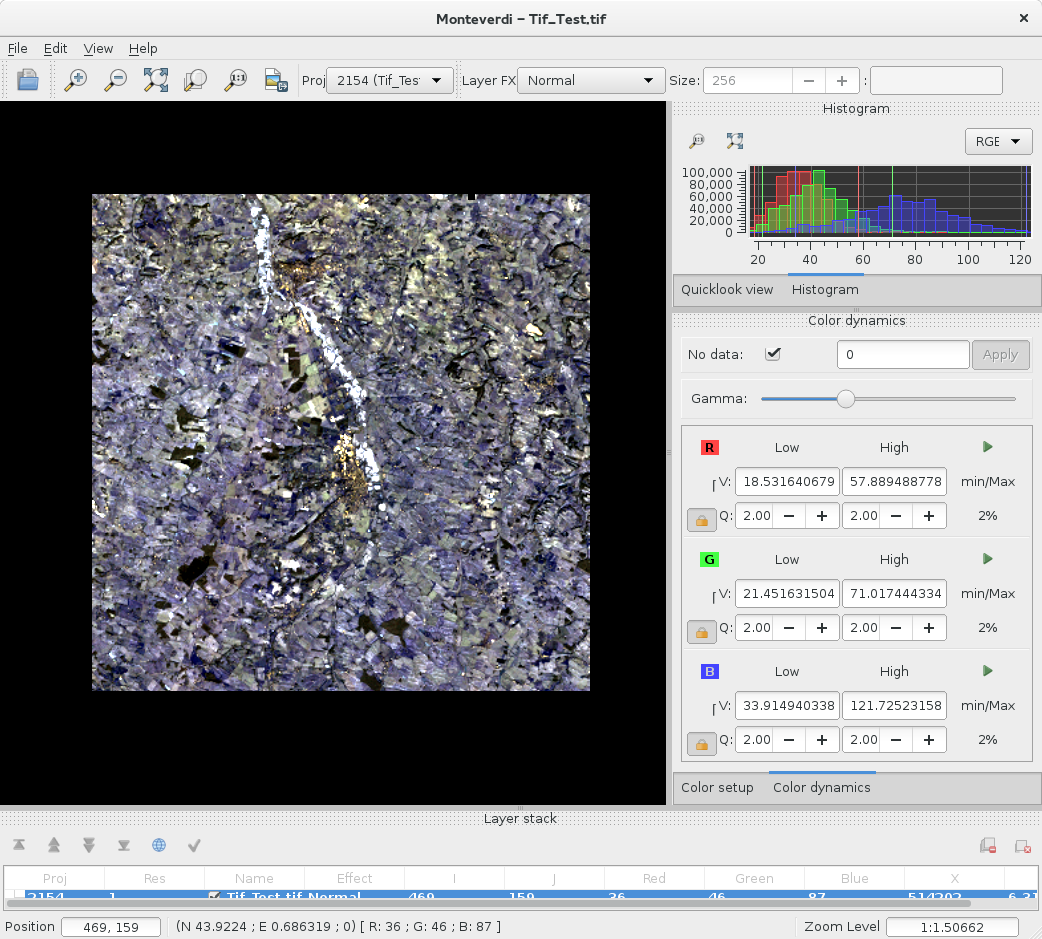
\includegraphics[width=1\textwidth]{Art/monteverdi-tif.png}
  \caption[]{Monteverdi}
  \label{fig:monteverdi}
\end{figure}

\begin{figure}[h]
  \center
  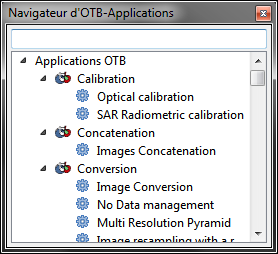
\includegraphics[scale=1]{Art/windows-mapla.png}
  \caption[]{OTB applications can be used from Monteverdi}
  \label{fig:windows-mapla}
\end{figure}

\begin{figure}[h]
  \center
  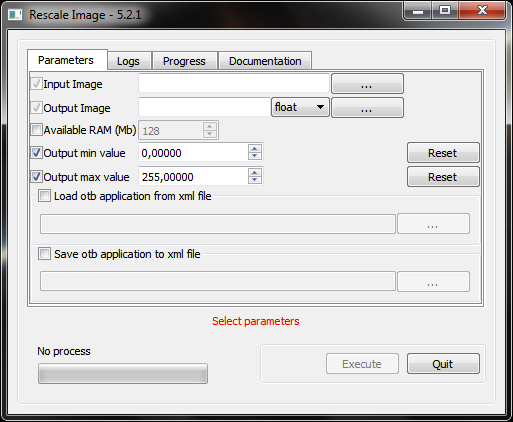
\includegraphics[scale=1]{Art/windows-otbgui.png}
  \caption[]{OTB Graphical User Interface}
  \label{fig:windows-otbgui}
\end{figure}

% En commentaire pour l'instant, c'est peut être un peu inutile puisqu'il n'y a
% aucune action associée en terme d'installation
\begin{comment}
\subsection{OTB depuis QGIS}

Les applications OTB sont disponibles depuis QGIS. Pour cela

Attention ! QGIS est livré avec ses propres binaires OTB. Les applications ainsi
ouvertes depuis QGIS sont souvent différentes de celles installée ci-dessus, car
il s'agit typiquement d'une version plus ancienne.
Éventuellement, il est possible de remplacer l'OTB livrée avec QGIS en supprimant
ou écrasant les fichiers dans \texttt{}.

\begin{figure}[h]
  \center
  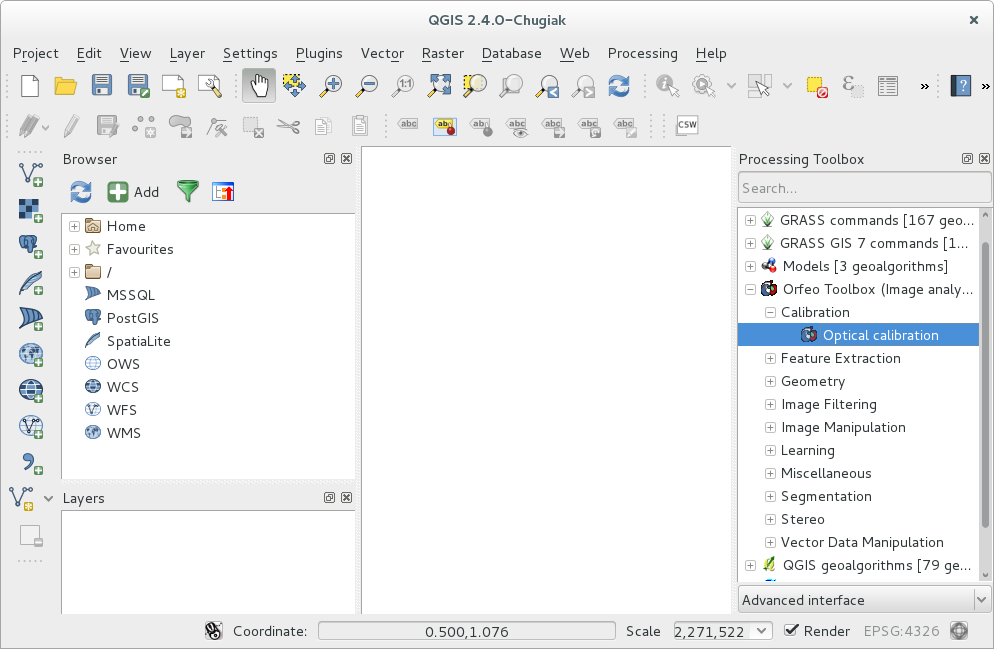
\includegraphics[width=1\textwidth]{Art/qgis-otb.png}
  \caption[]{Intégration QGIS - OTB}
  \label{fig:otb-qgis}
\end{figure}
\end{comment}

\clearpage
\section{Linux (Ubuntu example)}

This section explains how to install the tools in a Linux environment like Ubuntu. This procedure can also be used on other Linux distributions by using the appropriate package manager (dnf, yum,
emerge, pacman\ldots)

\subsection{QGis}
QGis can be installed via a command line like:
\begin{verbatim}
sudo apt-get install qgis
\end{verbatim}

\subsection{Dependencies installation}
Before installing the self-extracting Linux binary for OTB, several system dependencies have to be installed. In a terminal, type the following:
\begin{verbatim}
sudo apt-get install libx11-6 libxext6 libxau6 libxxf86vm1 libxdmcp6 libdrm2
\end{verbatim}
or the equivalent for other distributions.

You will need the libgl1 and libglu1 libraries, which have different implementations (MESA, FGLRX, NVIDIA, etc.). If you don't already have these libraries, you can use the MESA implementation:
\begin{verbatim}
sudo apt-get install libgl1-mesa-glx libglu1-mesa
\end{verbatim}

\subsection{Install OTB and Monteverdi}
Download the self-extracting binary for Linux (64 bits), available at:
\begin{center}
\url{https://www.orfeo-toolbox.org/download}
\end{center}

The self-extracting binary will extract itself in the current directory. First, the archive has to be made executable, and then it can be run:
\begin{verbatim}
chmod +x OTB-5.6.1-Linux64.run
./OTB-5.6.1-Linux64.run
\end{verbatim}

The executable binaries will be inside the 'bin' directory, and you can put this directory in your PATH variable if you want to. 

There are also scripts which set all the environment variables to allow to run Monteverdi and Mapla:
\begin{verbatim}
cd OTB-5.6.1-Linux64
./monteverdi.sh
./mapla.sh
\end{verbatim}

\subsection{Test the installation}
Once the installation is done, OTB applications can be run in several ways. Check that you have a working installation with the following steps:
\begin{enumerate}

\item Try to open a tif image in Monteverdi (see
figure~\ref{fig:monteverdi}). A demonstration tif image is available here: \url{https://git.orfeo-toolbox.org/otb-data.git/blob/HEAD:/Examples/QB\_Toulouse\_Ortho\_PAN.tif}.

\item The application browser is available from the ``View'' menu 
$\rightarrow$ "OTB-Applications browser".
(see figure \ref{fig:windows-mapla}).

\item Run an application using the terminal, for instance
\texttt{otbgui\_Rescale}. (see figure \ref{fig:windows-otbgui}).

\end{enumerate}

\clearpage
\section{Mac OS X}

The software can also be installed on Mac OS X.

First install QGIS using the instructions for Mac OS X on the official site. To install OTB and  Monteverdi download 
OTB-5.6.1-Darwin64.run from \url{https://www.orfeo-toolbox.org/download/}.

This is a self-extracting binary which extracts itself in the current directory. Testing the installation is done like in the Linux case.

\end{document}
